	\documentclass[12pt,a4paper]{article}
	\usepackage[a4paper, left=3.5cm, right=2cm, top=2.5cm, bottom=1.2cm]{geometry}
	\usepackage[utf8]{inputenc}
	%\usepackage[T1]{fontenc}
	\usepackage[ngerman]{babel}
	\usepackage{graphicx} 
	\usepackage{hyperref} 
	\usepackage{pgfplots}
	\usepackage{listings}
	\lstset{numbers=left, numberstyle=\tiny, numbersep=5pt}
	\lstset{language=Java}
	%\usepackage[german]{algorithm2e}
	%\glqq \grqq{}
	\usepackage{tikz}
	\usetikzlibrary{positioning,shadows,arrows}

	\title{Vier Gewinnt}
	\author{Florian Tünte}
	
	\begin{document}
	\pagenumbering{gobble}
	\maketitle
	\newpage
	\tableofcontents
	\newpage
	\pagenumbering{arabic}
	\section{Einleitung}
	Das Spiel \glqq Vier Gewinnt\grqq{} erscheint auf den ersten Blick relativ simpel. Nahezu jeder hatte schon Kontakt mit diesem Spiel und hat es sicher einmal oder auch viele Male gespielt. Egal ob auf einem Blatt Papier im Unterricht, mit kleineren oder größeren Spielen aus Plastik, es ist immer ein faszinierendes Spiel für zwei Personen. Es ist nicht so simpel wie z.B. Tic-Tac-Toe, bei dem es unter geübten Spielern immer in einem Unentschieden endet. Bei dem Spiel \glqq Vier Gewinnt\grqq{} geht es im Wesentlichen um das Aufbauen von Fallen, die man dann ausnutzen kann, um zu gewinnen, wenn der Gegenspieler diese ausgelöst hat. Nachdem ich schon einmal ein \glqq Tic-Tac-Toe\grqq{} Spiel mit unbesiegbarem Computergegner programmiert hatte.
	%auf der Suche nach einem anspruchsvollerem Spiel; die Wahl fiel auf Vier gewinnt 
	\footnote{\url{https://github.com/boba2fett/TicTacToe}}
	, war mir klar, dass ich bei der Facharbeit dies mit einem  \glqq Vier Gewinnt\grqq{} Spiel umsetzen könnte.
	\section{Vier Gewinnt}
	\subsection{Spielidee}
	Die Grundidee des \glqq Vier Gewinnt\grqq{} Spieles ist es, vier der eigenen Spielsteine bzw. Symbole in eine Reihe zu bringen.
	Dabei ist es egal, ob dies horizontal, vertikal oder diagonal erreicht wird.
	Es spielen immer zwei Spieler gegeneinander, die abwechselnd einen Spielstein von oben in das Spielfeld einfügen, der dann so lange herunterfällt, bis er auf das Ende des Spielfeldes oder einen anderen Spielstein stößt.
	%einwerfen, herabfallen, setzen
	Sobald zum ersten Mal vier Spielsteine eines Spielers eine Reihe bilden, endet das Spiel und der betreffende Spieler gewinnt.
	Das Spielfeld in der Grundversion ist ein 7x6 Feld. Grundsätzlich sind aber auch größere und kleinere Spielfelder möglich.
	\footnote{Lehmann, Jörg \glqq Vier gewinnt\grqq{} \url{http://www.brettspiele-report.de/vier-gewinnt/} Stand: 01.05.2019}
	\subsection{Implementation}
	Direkt am Anfang habe ich ein Github-Repository angelegt und das Grundspiel Vier Gewinnt programmiert.\footnote{\url{https://github.com/boba2fett/viergew}} Das wichtigste dabei war zu erkennen das jemand gewonnen hat und zu die Möglichkeit mit zwei Spielern in die verschiedenen Spalten zu setzen.
	Nach der Umsetzung des kompletten Projekts versuchte ich die Laufzeit etwas zu senken, indem ich eine eigene Klasse VierLogik erstellte, an deren Objekten die Simulationen durchgeführt wird, um es mehr abzutrennen und die redundante Speicherung der bisherigen Züge zu vermeiden. Am Ende des Entwicklungsprozesses habe ich eine grafische Oberfläche erstellt, um das Spiel effizienter zu testen bzw um es ansprechender zu machen. Dabei fiel mir auf, dass die Funktion zu sehen, mit welchen Feldern man gewonnen hat, sehr praktisch ist, da sonst schnell der Überblick und die Lust am Spielen verloren geht. In der Konsolen-Version waren die Tester nur wenig begeistert.
	Damit sieht das Implementationsdiagramm ohne die Klasse, die für die Ki zuständig ist, wie folgt aus:
\begin{figure}[h]
	\centering
	\label{Impementationsdiagramm}
	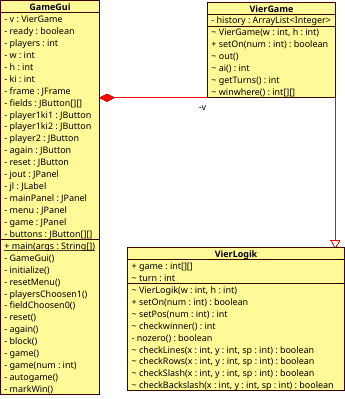
\includegraphics[width=0.7\linewidth, height=0.4\textheight]{maybe/Klassendiagramme}
	\caption{Klassendiagramme}
	\label{fig:klassendiagramme}
\end{figure}
\\
	\subsection{Das Programm}
	Wie startet man das Programm? Es ist relativ simpel. Wenn java installiert ist sollte ein Doppelklick auf die jar-Datei genügen. Andernfalls muss java noch installiert werden. Die jar Datei ist direkt im viergew Verzeichnis zu finden. Die grafische Oberfläche öffnet sich und man hat die Gelegenheit sich für eine Spielfeldgröße zu entscheiden. Danach muss man auswählen, ob der Computer die Rolle des Anfangenden übernimmt oder nicht oder ob man lieber zu zweit spielt.
	\section{Die KI (künstliche Intelligenz)}
	\subsection{Taktik der KI}
	Die Taktik der KI ist natürlich zu gewinnen oder eine (unmittelbare) Niederlage zu verhindern. Dazu wird ein Minimax-Algorithmus genutzt, um die beste Entscheidung zu treffen. Bei diesem Verfahren durchläuft der Algorithmus einen Suchbaum, der bei der maximalen Suchtiefe jedem Ergebnis einen Wert zuweist oder, wenn schon vorher ein Sieg oder eine Niederlage auftritt, diesen jeweils einen positiven bzw. negativen Wert zuordnet. Bei der Auswertung wird dann immer das Minimum der gegnerischen Züge gewertet und das Maximum der eigenen, so dass jeder Spieler ein \glqq perfektes \grqq{} Spiel spielt. Des Weiteren bevorzugt der Algorithmus einen schnellen Sieg bzw. eine spätere Niederlage.\\
	Neben dem Minimax-Algorithmus könnten auch vorberechnete Eröffnungszüge genutzt werden, aber diese unterscheiden sich für jede Spielfeldgröße. Einige Spiele gelten dadurch auch schon als gelöst. Das Diagramm zeigt wer bei einem perfekten Spiel gewinnt (+ der anfangende Spieler gewinnt, - der Gegenspieler gewinnt, = Unentschieden), wenn man die Höhe und Breite variiert.
	\begin{figure}[h]
		\centering
		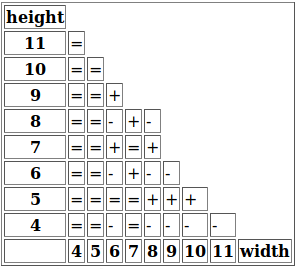
\includegraphics[width=0.5\linewidth, height=0.3\textheight]{w-h-viergew}
		\caption{Feldgrößen und wer gewinnt}
		\label{fig:w-h-viergew}
		\footnote{Tromp, John  \glqq John's Connect Four Playground \grqq{} \url{http://tromp.github.io/c4/c4.html} Stand: 01.05.2019}
	\end{figure}
\\
	\subsection{Schwächen}
	Theoretisch sind der KI mit dem Minimax-Algorithmus nur Grenzen durch die Rechenleistung des Computers bzw. die Tiefe der Simulation gesetzt.
	
	\subsection{Implementation}
	Zunächst auch zu dieser Klasse das Implementationsdiagramm.
\begin{figure}[h]
	\centering
	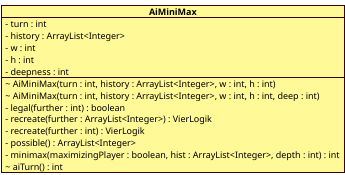
\includegraphics[width=0.7\linewidth, height=0.3\textheight]{maybe/KlassendiagrammKI}
	\caption{Klassendiagramm Klasse AiMiniMax}
	\label{fig:klassendiagrammki}
\end{figure}
	\\Die wichtigste Frage ist zunächst, wie der Computer \glqq denken\grqq{} soll. Als ich im Internet recherchiert habe stieß ich schnell auf den Minimax-Algorithmus. Die Grundidee ist, dass jeder Spieler ein  \glqq perfektes\grqq{} Spiel spielt.\footnote{Wikimedia Foundation Inc. \glqq Minimax\grqq{} \url{https://en.wikipedia.org/wiki/Minimax} Stand: 12.05.2019} Hier verwendet ist aber eine Abgewandelte Form, da manche Pfade nicht weiter verfolgt werden, wenn sie nicht auf das Ergebnis einfließen. Für die Implementation habe ich mich dann am Wikipedia Pseudocode orientiert. Das interessante ist, dass ich zuerst auf den englischen Artikel gestoßen bin und dass sich der Pseudocode deutlich unterscheidet.\footnote{Wikimedia Foundation Inc. \glqq Minimax\grqq{} \url{https://en.wikipedia.org/wiki/Minimax} Stand: 12.05.2019}\\
		Die KI ist in der Klasse AiMiniMax beherbergt. Die dabei wichtigen Methoden sind zum einen die Methoden zum Erzeugen von \textit{VierLogik} Objekten, an denen die Simulationen durchgeführt werden, und zum anderen die Umsetzung des MiniMax-Algorithmus. Der Aufruf aus \textit{VierGame} benutzt die Methode \textit{aiTurn}. In dieser Methode wird jeder Möglichkeit auf ein Feld zu setzen ein Wert durch den MiniMax-Algorithmus zugeordnet und danach wird auf das Feld mit dem höchsten evaluierten Wert gesetzt bzw. auf eines der Felder mit dem höchsten evaluierten Wert. Das Herz der KI ist aber der MiniMax-Algorithmus. Der Aufruf erfolgt damit, dass der Zug günstig für den Gegenspieler ist (minimierend für die KI), weil der Zug der KI ja schon für jedes der verfügbaren Felder gemacht wurde, um jedem dieser Felder mit dem Aufruf von \textit{minimax(false,hist,deepness);}einen Wert zuzuweisen (\textit{hist} bestehend aus dem Feld für das evaluiert wird). Wenn es hier bei einer der durchprobierten Möglichkeiten für den Gegenspieler zu setzen zu einem Sieg des Gegenspielers kommt, wird ein negativer Wert zugewiesen, der \textit{depth} entspricht und zurückgegeben wird. Dies sorgt dafür, dass eine spätere Niederlage besser bewertet wird als eine frühe Niederlage. Bei einem Unentschieden ist der entsprechende Wert 0. Wenn nichts davon eingetreten ist, wird der entsprechende Zug in \textit{history} gespeichert und der Algorithmus beginnt den nächsten Zug des Spielers zu bewerten. Hier gilt das Umgekehrte, da es den Spieler maximiert. Ein früher Sieg bekommt eine sehr positive Bewertung	%durch Testspieler ist mir aufgefallen, dass die KI sich zu langsam für eine Sieg entscheidet, Im der weiteren Quelltexterstellung/generierung ist aufgefallen, dass die KI denkt, sie hätte nur ein kleineres Feld anstatt des vorhanden 8x8 Spielfeldes.
	 und im nächsten Aufruf ist es wieder minimierend. Wenn die maximale Suchtiefe erreicht ist, wird 0 zurückgegeben und diese Reihenfolge an Zügen wird wie ein Unentschieden behandelt.
	\subsubsection{1. Beispiel}
	Nun betrachten wir eine Beispielsituation, wie sie vorkommen könnte und sehen uns genauer an, wie die KI ihre Entscheidung trifft. Diese werden durchgeführt auf einem kleinen Feld von der Größe 4x4 und die KI soll einen Verteidigungszug machen. Damit das Log nicht zu lang wird, wird die die KI auf eine Suchtiefe von 4 begrenzt. Die Ausgaben werden erzeugt durch die Klasse \textit{AiMiniMaxPrint}.
	Gegeben ist folgende Situation (folgendes sind Screenshots aus dem Programm):
\begin{figure}[h]
	\centering
	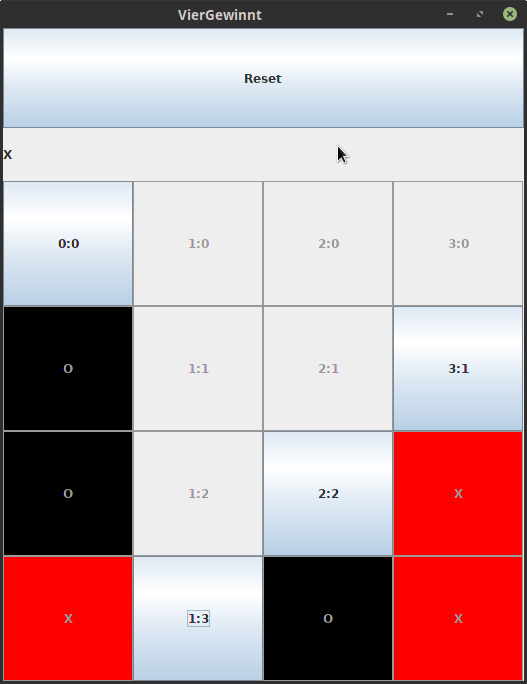
\includegraphics[width=0.4\linewidth, height=0.3\textheight]{maybe/fach0}
	\caption{Anfangs Situation}
	\label{fig:fach0}
\end{figure}
	\\Im folgenden setzt der Spieler beispielsweise gegen den Computer auf das Feld 3:1, um zu testen, ob er die Bedrohung erkennt.
\begin{figure}[h]
	\centering
	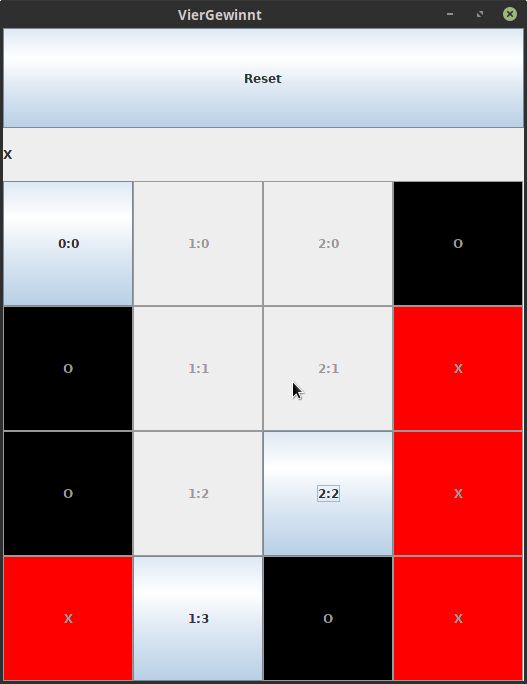
\includegraphics[width=0.4\linewidth, height=0.3\textheight]{maybe/fach1}
	\caption{KI erkennt Bedrohung}
	\label{fig:fach1}
\end{figure}
	\\Das Ergebnis: Der Computer erkennt die Bedrohung. Aber warum?\\
	Dazu sehen wir uns das generierte Log an. Zu finden unter /viergew/FachTex/maybe/fach0-1.
	\begin{lstlisting}[basicstyle=\sffamily]
0,3 Defeat
1,3 Defeat
2,3 Defeat
3,return 0
Evaluated Value 0
Consider 3
	\end{lstlisting}
	Aber was steht hier? Es werden alle Möglichkeiten durchprobiert, bis man in einer maximierenden Ebene auf einen Sieg oder in einer minimierenden Ebene auf eine Niederlage trifft. Zeile 1 zeigt, wenn der Computer auf 0 setzt, dass der Spieler mit dem Setzen auf 3 gewinnt. Also eine Niederlage für die KI. Zeile 2 und 3 zeigen das gleiche Ergebnis für den ersten Zug auf 2 oder 3. Zeile 4 hingegen macht deutlich, dass in den weiteren Stufen bis zur maximalen Suchtiefe weder der Spieler noch die KI durch ein perfektes Spiel gewinnt.
	\\
	\begin{figure}[h]
		\centering
		\label{fig:baumdiagramm1}
	\begin{tikzpicture}[
	max/.style={rectangle, draw=none, rounded corners=1mm, fill=blue, drop shadow,
		text centered, anchor=north, text=white},
	min/.style={circle, draw=none, fill=orange, circular drop shadow,
		text centered, anchor=north, text=white},
	beginn/.style={circle, draw=none, fill=red, circular drop shadow,
		text centered, anchor=north, text=white},
	level distance=0.5cm, growth parent anchor=south
	]
	\node (n) [max,sibling distance=9cm] {Anfang}
child{
	[sibling distance=5cm]
	node (c) [beginn] {0}
	child{
		[sibling distance=1.7cm]
		node (c1) [min] {1}
		child{[sibling distance=0.5cm]
			node (c11) [max] {1}
			child{
				node (c111) [min] {1}
			}
			child{
				node (c112) [min] {2}
			}
			child{
				node (c113) [min] {3}
				child{
					node (c113D) [min] {D}
				}
			}
		}
		child{[sibling distance=0.5cm]
			node (c12) [max] {2}
			child{
				node (c121) [min] {1}
			}
			child{
				node (c122) [min] {2}
			}
			child{
				node (c123) [min] {3}
				child{
					node (c123D) [min] {D}
				}
			}
		}
		child{[sibling distance=0.5cm]
			node (c13) [max] {3}
			child{
				node (c131) [min] {1}
			}
			child{
				node (c132) [min] {2}
			}
		}
	}
	child{
		[sibling distance=1.7cm]
		node (c2) [min] {2}
		child{[sibling distance=0.5cm]
			node (c21) [max] {1}
			child{
				node (c211) [min] {1}
			}
			child{
				node (c212) [min] {2}
			}
			child{
				node (c213) [min] {3}
				child{
					node (c113D) [min] {D}
				}
			}
		}
		child{[sibling distance=0.5cm]
			node (c12) [max] {2}
			child{
				node (c221) [min] {1}
			}
			child{
				node (c222) [min] {2}
			}
			child{
				node (c223) [min] {3}
				child{
					node (c123D) [min] {D}
				}
			}
		}
		child{[sibling distance=0.5cm]
			node (c23) [max] {3}
			child{
				node (c231) [min] {1}
			}
			child{
				node (c232) [min] {2}
			}
		}
	}
	child{
		node (c3) [min] {3}
		child{
			node (c3d) [min] {D}
		}
	}
}
	;
	\end{tikzpicture}
	\caption{Baumdiagramm zur Entscheidung auf 0 zu setzen}
	\end{figure}
	\\\\
	Hier ist das Baumdiagramm zu 0 als ersten Zug der KI zu sehen, in dem alle Simulationen angeführt sind, die gemacht werden. Endet ein Pfad im Nichts, ist die maximale Tiefe erreicht, also im Ergebnis ein Unentschieden. Steht ein D am Ende eines Pfades ist es eine Niederlage. Blau eingefärbte Knoten sind Maximierende und Orange eingefärbte Minimierende. Fangen wir von links an.\\ Die Maximale Tiefe ist erreicht, also ist der Wert für den Pfad 0-1-1 (Von oben nach unten gelesen) erst mal das Maximum 0. Der nächste Wert von rechts ist wieder 0, also keine Veränderung. Der darauf folgende ist eine Niederlage, aber da es ein maximierender Knoten ist, zählt hier das Maximum, 0. Die beiden Knoten daneben liefern kein anderes Ergebnis und dadurch wird der Wert des minimierenden Knotens 0-1 auch 0. Für den Knoten 0-2 gilt das gleiche. Der Knoten 0-3 mündet direkt in eine Niederlage und damit einen negativen Wert (hier -2, da Wert=-Suchtiefe+aktuelle Tiefe). Das Minimum von 0-1, 0-2 und 0-3 ist also -2.\\
	Bei dem Start mit dem Knoten 3 ergibt sich nachher ein Wert von 0, der dann den anderen Ergebnissen (0,1,2) bevorzugt wird. Am Ende wird im Log noch niedergeschrieben, dass beim Wert 0 das Feld 3 eine Möglichkeit ist, welches dann auch ausgewählt wird.
	\subsubsection{2.Beispiel}
	Beim zweiten Beispiel wird nun eine Situation herbeigeführt, bei dem wir in der Zwickmühle sitzen.
	\begin{figure}[h]
		\centering
		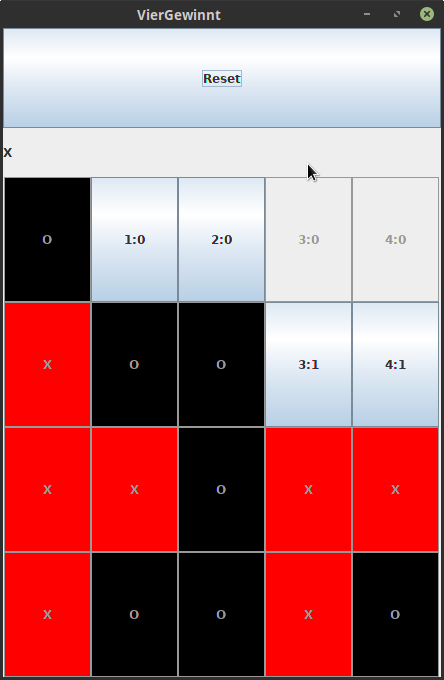
\includegraphics[width=0.4\linewidth, height=0.3\textheight]{maybe/fach2}
		\caption{Anfangssituation}
		\label{fig:fach2}
	\end{figure}
	\\Nun setzen wir als Spieler auf 2:0, um nicht das Spiel zu verlieren.
	\begin{figure}[h]
		\centering
		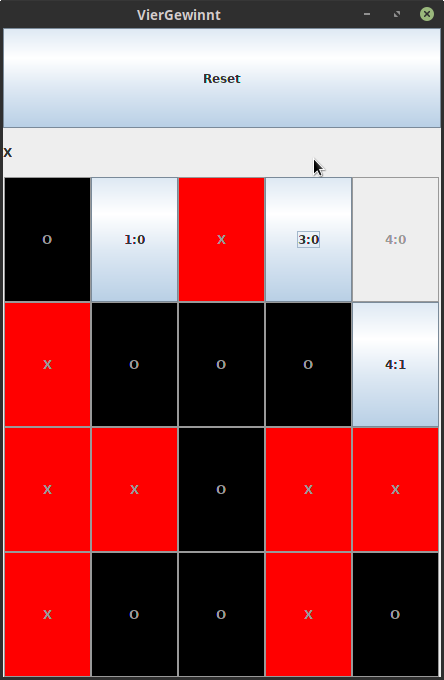
\includegraphics[width=0.4\linewidth, height=0.3\textheight]{maybe/fach3}
		\caption{KI trifft gute Entscheidung}
		\label{fig:fach3}
	\end{figure}
	\\Und die KI setzt auf 3:1 und wir haben keine Chance mehr zu gewinnen. Setzen wir auf 4:1, setzt die KI im nächsten Zug auf 4:0 und gewinnt. Setzten wir hingegen nicht auf 4:1, setzt die KI auf dieses Feld und gewinnt ebenfalls.
	Schauen wir uns nun wieder den Suchbaum an. Er geht hervor aus fach2-3 (/viergew/FachTex/maybe/fach2-3).\\
	\begin{figure}[h]
	\centering
	\label{fig:baumdiagramm2}
	\begin{tikzpicture}[
	max/.style={rectangle, draw=none, rounded corners=1mm, fill=blue, drop shadow,
		text centered, anchor=north, text=white},
	min/.style={circle, draw=none, fill=orange, circular drop shadow,
		text centered, anchor=north, text=white},
	beginn/.style={circle, draw=none, fill=red, circular drop shadow,
		text centered, anchor=north, text=white},
	level distance=0.5cm, growth parent anchor=south
	]
	\node (n) [max,sibling distance=9cm] {Anfang}
	child{
		[sibling distance=5cm]
		node (c) [beginn] {3}
		child{
			[sibling distance=1.7cm]
			node (c1) [min] {1}
			child{[sibling distance=0.5cm]
				node (c13) [max] {3}
				child{
					node (c134) [min] {4}
					child{
						node (c1344) [max] {4}
						child{
							node (c1344W) [max] {W}
						}
					}
				}
			}
			child{[sibling distance=0.5cm]
				node (c14) [max] {4}
				child{
					node (c14W) [max]{W}
				}
			}
		}
		child{
			[sibling distance=1.7cm]
			node (c3) [min] {3}
			child{[sibling distance=0.5cm]
				node (c31) [max] {1}
				child{
					node (c314) [min] {4}
					child{
						node (c3144) [max] {4}
						child{
							node (c3144W) [max] {W}
						}
					}
				}
			}
		child{[sibling distance=0.5cm]
			node (c34) [max] {4}
			child{[sibling distance=0.5cm]
				node (c34W) [max] {W}
			}
		}
		}
		child{[sibling distance=2cm]
			node (c4) [min] {4}
			child{[sibling distance=1cm]
				node (c41) [max] {1}
				child{
					node (c413) [min] {3}
					child{
						node (c4134) [max] {4}
						child{
							node (c4134W) [max] {W}
						}
					}
				child{
					node (c4143) [max] {3}
					child{
						node (c4143T) [max] {T}
					}
				}
				}
			}
		child{[sibling distance=1cm]
			node (c43) [max] {3}
			child{
				node (c431) [min] {1}
				child{
					node (c4314) [max] {4}
					child{
						node (c4314W) [max] {W}
					}
				}
			}
		child{
			node (c434) [min] {4}
			child{
				node (c4341) [max] {1}
				child{
					node (c4341T) [max] {T}
				}
			}
		}
		}
			child{
				node (c44) [max] {4}
				child{
					node (c44W) [max] {W}
				}
			}
		}
	}
	;
	\end{tikzpicture}
	\caption{Baumdiagramm zur Entscheidung auf 3 zu setzen}
	\end{figure}
	\\
	Oben haben wir nun die Wahl des Feldes 3 die nächste Ebene ist minimierend. Auf der nächsten Ebene ist aber wieder alles Maximierend und es tritt bei jeder Möglichkeit, durch einen schlauen Zug, ein Sieg für die KI ein. Der errechnete Wert ist dabei dann 3 (Suchtiefe - aktuelle Suchtiefe) und dieser Wert wird von keiner der anderen möglichen Felder übertroffen. \\
	Hier das weitere Spiel bis zum Sieg der KI (weiteres Log auch unter fach3-4):\\
	\begin{figure}[h]
		\centering
		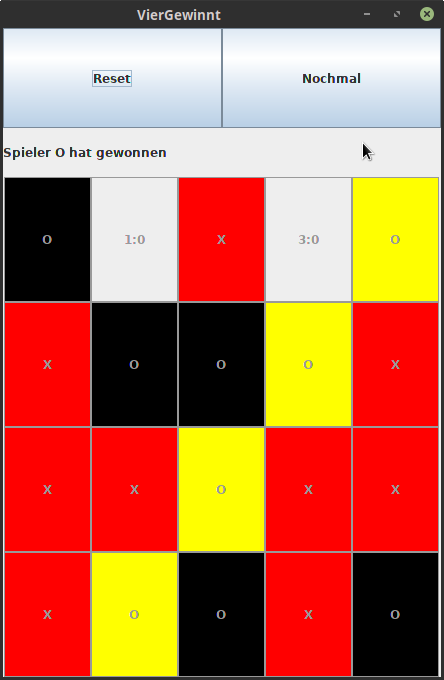
\includegraphics[width=0.4\linewidth, height=0.3\textheight]{maybe/fach4}
		\caption{KI gewinnt}
		\label{fig:fach4}
	\end{figure}
	\\
	\subsection{Effizienzbetrachtung}
	Um mehr Züge zu simulieren, ist erheblich mehr Rechenleistung erforderlich. Die Komplexität steigt nahezu exponentiell, aber je weiter das Spiel fortgeschritten ist und je weniger Möglichkeiten es gibt, desto schneller wird der Algorithmus. Ich habe Simulationen mit verschiedenen Feldgrößen durchgeführt und habe den ersten Zug von der KI berechnen lassen. Dabei habe ich die Zeit gemessen und darauf basierend passende Suchtiefen gewählt, um die Zeit bei weniger als 10 Sekunden zu belassen. Hätte ich die vordefinierten Pfade genommen, wäre deutlich an Rechenzeit gespart worden, jedoch bräuchte man zum Erstellen dieser sehr lange bzw. würde es den Rahmen dieser Facharbeit sprengen. Auch wäre es möglich anstatt der VierLogik Klasse einfach nur kopierte Arrays zu verwenden, aber dabei ist es schwer darauf zu achten, dass keines dieser Arrays verändert wird.\\
	Aber nun zur Effizienz bei verschiedenen Feldgrößen. Da die Höhe nicht so ausschlaggebend ist, wird hier nur betrachtet, wie sich die Ausführungszeit verändert, wenn die Suchtiefe und die Feldbreite variiert werden. Die KI versucht in jedem Fall den ersten Zug eines Spieles zu berechnen.\\
	Im Folgenden sind die Graphen der Ausführungszeit im Bezug auf die Suchtiefe dargestellt. Von oben nach unten mit den Feldbreiten 9,7,5. Es fällt deutlich auf, dass bis zu einer Suchtiefe von 5 kaum Unterschiede in der Rechenzeit auftreten. Von da an werden die Unterschiede pro weiterer Suchtiefe immer größer und steigen exponentiell. Der Wert für die Feldbreite 9 und Suchtiefe 9 fehlt, da ich die Messung nach 2 Stunden abgebrochen habe, Die Tests wurden durchgeführt mit der Klasse Testing.\\
		\begin{figure}
			\centering
			\label{fig:graph1}
		\begin{tikzpicture}
		\begin{axis}[xlabel=Suchtiefe,ylabel=Rechenzeit in $s$]
		\addplot coordinates{%5
			(1,0.002)
			(2,0.001)
			(3,0.007)
			(4,0.027)
			(5,0.022)
			(6,0.122)
			(7,0.451)
			(8,2.104)
			(9,10.888)
		};
		\addplot coordinates{%7
			(1,0.0)
			(2,0.001)
			(3,0.003)
			(4,0.022)
			(5,0.164)
			(6,1.151)
			(7,8.182)
			(8,55.315)
			(9,389.38)
		};
		\addplot coordinates{%9
			(1,0.001)
			(2,0.001)
			(3,0.011)
			(4,0.099)
			(5,0.904)
			(6,8.096)
			(7,73.896)
			(8,653.781)
		};
		\legend{$5$,$7$,$9$}
		\end{axis}
		\end{tikzpicture}
		\caption{Relation Spielfeldbreite zu Ausführungszeit}
		\end{figure}
	\\Vielleicht wäre es auch eine Beschleunigung,wenn man keine Tiefensuche benutzt, sondern eine, die erst in die Breite sucht, da dort Siege oder Niederlagen für die aktuelle Ebene schon Ausschlaggebend sein kann. Diese Idee ist mir leider erst später gekommen, aber dennoch werde ich diese Idee in dem Github Repository eventuell noch umsetzen. Auch eine Abtrennung der Ergebnis Berechnung könnten noch in einen anderen Thread verlagert werden, um das einfrieren der grafischen Oberfläche zu verhindern. Auch ein Netzwerkspiel, wie bei dem TicTacToe Spiel wäre möglich, wobei dieses auch nicht ganz ausgereift ist.
	\section{Künstliche Intelligenz}
	\subsection{Definition}
	Das große Problem beim Begriff künstliche Intelligenz ist, dass es keine allgemeingültige Definition von Intelligenz gibt. Eine Möglichkeit ist es, Intelligenz als Fähigkeit Probleme zu lösen zu sehen. Darunter berücksichtigt wäre auch, dass es verschiedene Arten von Intelligenz gibt. So beschreibt es die \glqq Theorie der multiplen Intelligenzen \grqq{} von Howard Gardner. So habe jeder Mensch eine Mischung aus sieben Intelligenzarten.\footnote{Bulenda, Max \glqq Künstliche Intelligenz: Definition, Erklärung und Beispiele \grqq{}\url{https://simplyki.de/kuenstliche-intelligenz-definition-erklaerung-und-beispiele/} Stand: 10.05.2019} 
	Darauf achtend schauen wir uns den Wikipedia Artikel an, da dort meistens eine gesellschaftlich anerkannte Definition steht.\glqq Künstliche Intelligenz (KI, auch Artifizielle Intelligenz (AI bzw. A. I.), englisch artificial intelligence, AI) ist ein Teilgebiet der Informatik, welches sich mit der Automatisierung intelligenten Verhaltens und dem Maschinellen Lernen befasst. \grqq{} \footnote{Wikimedia Foundation Inc. \glqq Künstliche Intelligenz \grqq{} \url{https://de.wikipedia.org/wiki/K\%C3\%BCnstliche_Intelligenz} Stand: 10.05.2019 }
	Etwas ähnliches  ist auch im Gabler Wirtschaftslexikon zu finden: \glqq Erforschung intelligenten Problemlösungsverhaltens sowie die Erstellung intelligenter Computersysteme. Künstliche Intelligenz (KI) beschäftigt sich mit Methoden, die es einem Computer ermöglichen, solche Aufgaben zu lösen, die, wenn sie vom Menschen gelöst werden, Intelligenz erfordern. \grqq{} \footnote{Prof. Dr. Richard Lackes und Dr. Markus Siepermann \glqq Künstliche Intelligenz (KI) \grqq{} \url{https://wirtschaftslexikon.gabler.de/definition/kuenstliche-intelligenz-ki-40285} Stand: 10.05.2019 }
	Und auch bei Spektrum steht etwas ähnliches: \glqq Die künstliche Intelligenz (Abk. KI, \textit{E} artificial intelligence, Abk. AI) ist ein Teilgebiet der Informatik, welches sich mit der Erforschung von Mechanismen des intelligenten menschlichen Verhaltens befaßt (Intelligenz). Dieses geschieht durch Simulation mit Hilfe künstlicher Artefakte, gewöhnlich mit Computerprogrammen auf einer Rechenmaschine (Computersimulation).\grqq{} \footnote{Wichert, Andreas \glqq Künstliche Intelligenz \grqq{} \url{https://www.spektrum.de/lexikon/neurowissenschaft/kuenstliche-intelligenz/6810} Stand: 10.05.2019 }
	Dem entsprechend kann man sagen, dass es sich wohl um die Nachahmung von menschlicher Intelligenz handelt, die durch Computersimulation oder andere Mechanismen erreicht wird.\\
	Damit lässt sich auch für einen Computergegner der Begriff künstliche Intelligenz wählen, da hier durch Computersimulation menschliche Intelligenz nachgeahmt wird.
	\subsection{Machine Learning}
	Ein Teilgebiet der künstlichen Intelligenz ist das Machine Learning, Maschinelles Lernen oder nur ML. Dabei geht es darum, aus vorhandenen Daten Muster und Gesetzmäßigkeiten abzuleiten, die dann bei ähnlichen Daten verwendet werden können. Solche lernenden Systeme können über verschiedene Wege angelernt werden, aber vor allem die Fortschritte im Bereich Big Data gaben diesem Themenfeld  eine enorme Bedeutung, da nun viele Daten zur Verfügung stehen, an denen gelernt werden kann.\footnote{Luber, Stefan \glqq Was ist Machine Learning? \grqq{} \url{https://www.bigdata-insider.de/was-ist-machine-learning-a-592092/} Stand:11.05.2019}
	\subsection{Aktueller Stand}
	Das heutige Leben wäre anders, wenn man auf künstliche Intelligenz verzichten würde. Das mag naheliegend sein bei Google Übersetzer oder anderer Sprachverarbeitung. Aber auch bei Verkehrsmitteln, wie Flugzeugen wird auf KI gesetzt. Man müsse also, um auf KI zu verzichten, mit einer Kutsche fahren. \footnote{Kersting, Pia \glqq Künstliche Intelligenz (KI): Der aktuelle Stand der Technik \grqq{} \url{https://lead-conduct.de/2017/11/21/kuenstliche-intelligenz-ki-der-aktuelle-stand-der-technik/} Stand:11.05.2019}
	Es sollte aber im Blick gehalten werden, dass KI unser Leben deutlich vereinfachen kann. So wurde schon 2018 bei der Google I/O demonstriert, wie es aussehen könnte, wenn der Google Assistant einen Termin für seinen Nutzer ausmacht.\footnote{Engelien, Marco \glqq Googles Assistant kann bald euren Friseur anrufen und einen Termin machen \grqq{} \url{https://curved.de/news/bei-anruf-google-der-assistant-macht-bald-termine-fuer-euch-ab-605280} Stand: 11.05.2019}
	Auch die Verfügbarkeit von Bibliotheken und Tutorials für KI oder ML ist gut. So gibt es Beispielsweise das von Google entwickelte open-source tensorflow Framework \footnote{\url{https://github.com/tensorflow/tensorflow}}, aber auch die Tutorials werden immer besser. Es gibt ein Spiel in dem man durch das Erlernen von ML gegen Außerirdische ankommen muss. Es befindet sich noch in der Alpha, ist aber ein guter Einstieg für python und ML, unter anderem mit verschiedenen python Bibliotheken, wie NumPy oder pandas.\footnote{\url{https://ml-scifi.com/}}
	\subsection{Ausblick}
	Im Folgenden werde ich darauf eingehen, was in der Zukunft noch auf uns zukommen könnte bzw. was jetzt schon möglich ist. Ein gutes Beispiel für die Ängste der Menschen liefern Filme mit alternativen Welten, die unserer ähneln. Als erstes Beispiel für eine lernende KI ist natürlich der Film \textit{Wargames} zu nennen. Darin erkennt die KI, dass Tic-Tac-Toe spielen immer nur im Unentschieden endet und überträgt dies auf einen thermonuklearen Krieg, in dem es auch keine Gewinner oder Verlierer gibt. Auch der Film \textit{I Robot} und die \textit{Terminator} Reihe spielen auf die große Angst der Menschen an, dass sich die Maschinen gegen uns wenden werden. Auch in Matrix scheint dies so zu sein, jedoch sollte hier auch die Vorgeschichte beachtet werden, in der die Menschen die Maschinen ablehnten. Es gibt auch andere Vertreter, in denen KI immer wieder auftaucht. In Spielen ist die Erzeugung von NPCs (nicht spielbarer Charakter) schon immer wichtig gewesen. Bei Brettspielen ist es eventuell noch möglich etwas zu simulieren, aber bei Shootern ist dies schon weniger möglich, so lassen manche Studios lieber die Mitstreiter verschwinden, als das sie eine wichtige Rolle im Kampf bekommen, weil sie sowieso nur im Weg stünden. Und jetzt mit den Möglichkeiten des ML könnten solche Dinge immer leichter umgangen werden.\\
	Ich denke im Allgemeinen entwickelt sich die KI zu unserem Nutzen. Auf die Gesetze der Robotik zurückgreifen wäre vielleicht eine Möglichkeit die Angst der Menschen zu mildern, aber es ist nur schwer abzuschätzen, ob KI uns irgendwann ersetzen wird oder nicht. Ob sie sich gegen uns auflehnen wird oder ob sie nur zu unserem Nutzen existieren wird. Sobald Quantencomputer und KI miteinander verbunden werden, muss sicherlich nochmal intensiver darüber nachgedacht werden.
	\subsection{Fazit}
	Am Ende der Facharbeit möchte ich noch einmal erwähnen, dass es immer eine Bereicherung ist mit \LaTeX{} einen Text zu schreiben und ich den Erfindern sehr dafür danke. es ist immer wieder eindrucksvoll, was mit \LaTeX{} alles möglich ist, wie die Baumdiagramme und der Graph. Die Klassendiagramme, die sie sehen wurden erstellt mit dem Programm \glqq Umbrello\grqq{}. Des weiteren habe ich nach dem komplette Entwicklungsprozess noch \textit{javadoc} erstellt. Die Dokumentation ist genauso wie der Quellcode und die Kommentare in Englisch gehalten, da dies auch bei deutschen Software Unternehmen so ist und jeder Quelltext, der auf Github ist auch für eine möglichst große Anzahl an Personen zur Verfügung stehen sollte. Ich denke das faszinierende am Programmieren ist das experimentieren und das niemals wirklich fertig mit etwas sein. Dieses Projekt hat mir außerdem noch einmal gezeigt, wie wichtig Tests sind. So viel mir ein gravierender Fehler in der KI erst auf, als meine Schwester das Programm testete.
	%programme verlinken
\end{document}

